\chapter{Captured gestures}
\label{chap:gestures}

The following images present the gestures captured in the data acquizition phase.

\begin{figure}
    \centering
    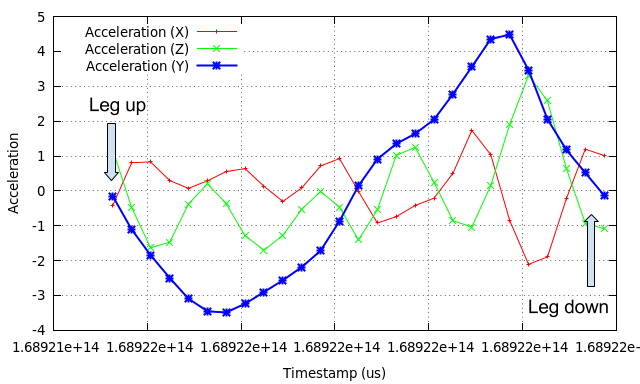
\includegraphics[width=0.7\textwidth]{src/img/xyz-stairs-down.png}
    \caption{Accelerometer data for going down a stair}
    \label{fig:xyz-stairs-down}
\end{figure}


\begin{figure}
    \centering
    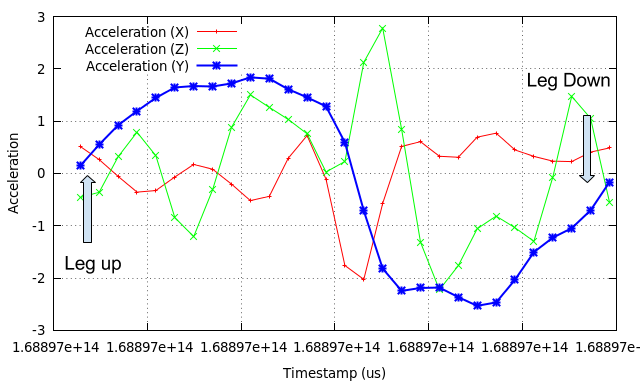
\includegraphics[width=0.7\textwidth]{src/img/xyz-stairs-up.png}
    \caption{Accelerometer data for going up a stair}
    \label{fig:xyz-stairs-up}
\end{figure}


\begin{figure}
    \centering
    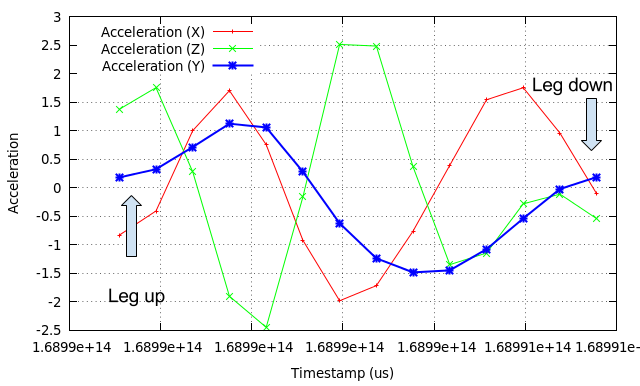
\includegraphics[width=0.7\textwidth]{src/img/xyz-walking.png}
    \caption{Accelerometer data for walking}
    \label{fig:xyz-walking}
\end{figure}


\begin{figure}
    \centering
    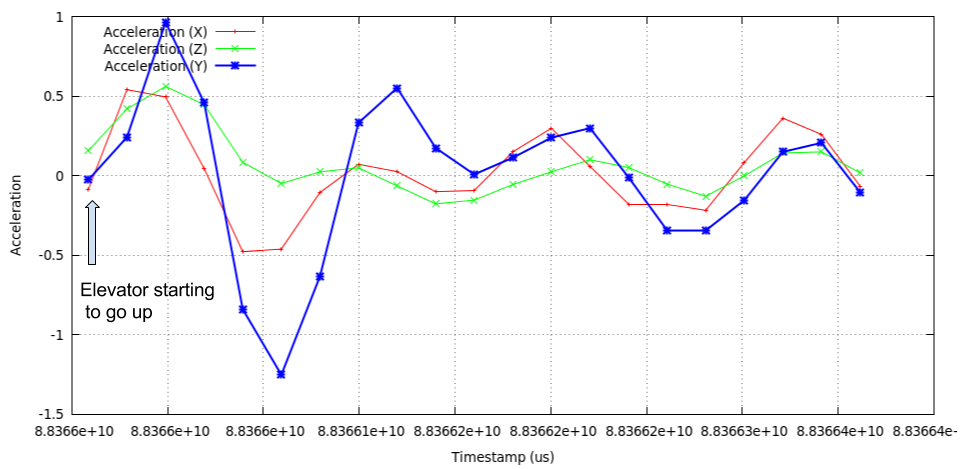
\includegraphics[width=0.7\textwidth]{src/img/xyz-elevator-up-start.png}
    \caption{Accelerometer data for elevator starting to go up}
    \label{fig:xyz-elevator-start}
\end{figure}

\begin{figure}
    \centering
    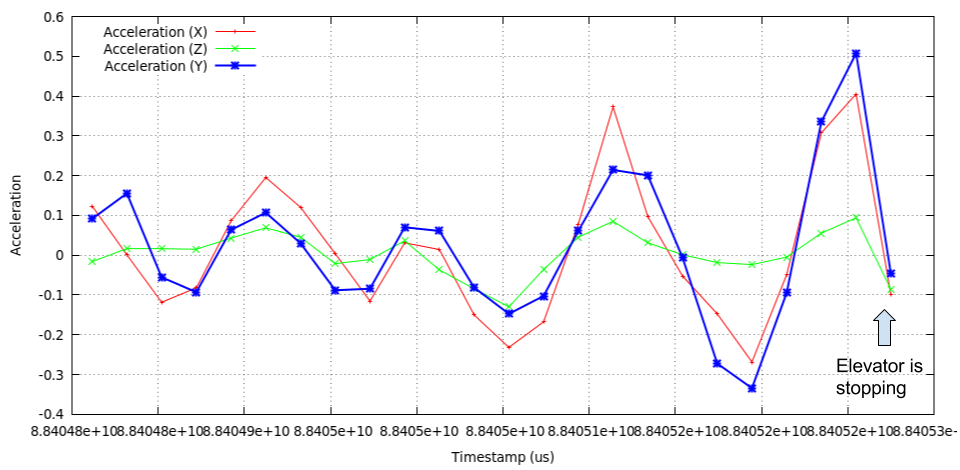
\includegraphics[width=0.7\textwidth]{src/img/xyz-elevator-up-stop.png}
    \caption{Accelerometer data for elevator stopping}
    \label{fig:xyz-elevator-stop}
\end{figure}

